\section{Results}\label{sec-results}
\subsection{Global Eye-Movement Analyses}\label{sub-sec-globaleyemovementanalysis}

This section presents the results of the global eye-movement analyses, examining reading patterns across entire subtitles. The analysis considers measures such as average fixation duration, total number of fixations, saccade length, and percentage of skipped subtitles. These measures provide insights into general reading approaches and the extent of reliance on subtitles under different audio conditions.

\subsubsection{Average Fixation Duration}\label{sub-sub-sec-averagefixation}

The analysis uncovered a main effect of the audio condition on
participants\textquotesingle{} average fixation duration, F(2, 18) =
12.34, p \textless{} .001, $\eta^2$ = .58. Pairwise contrasts (see \Cref{tab-03})
showed that when no audio was present, fixation durations were
significantly longer (M = 507.75 ms, SD = 147.02) compared to conditions
with either L1 audio (M = 290.25 ms, SD = 111.94) or L2 audio (M =
300.22 ms, SD = 111.11), ps \textless{} .01. Furthermore, no significant
differences were found between fixation durations for L1 and L2 audio
conditions, p \textgreater{} .05. Moreover, the subtitle language did
not significantly affect fixation duration, nor did the interaction
between audio condition and subtitle language, Fs \textless{} 1.

\begin{table}[!htbp]
\centering
\caption{Descriptive Statistics for Global Eye-Movement Measures.}
\label{tab-03}
\begin{threeparttable}

\begin{tabular}{lllll}
\toprule
\multicolumn{1}{p{2.5cm}}{Audio Condition} & 
\multicolumn{1}{>{\raggedright\arraybackslash}p{2.5cm}}{Subtitle Language} & 
\multicolumn{1}{p{2.5cm}}{Average Fixation Duration (ms)} &
\multicolumn{1}{p{2.5cm}}{Total Number of Fixations} & 
\multicolumn{1}{p{2.5cm}}{Average Saccade Length (\%)} \\
\midrule
L1 Audio & Arabic & 315.04 (105.74) & 3377 & 9.43 (9.40) \\
L1 Audio & Spanish & 265.45 (118.13) & 7663 & 10.63 (11.40) \\
L2 Audio & Arabic & 311.62 (106.81) & 2320 & 8.84 (6.52) \\
L2 Audio & Spanish & 288.82 (115.40) & 4740 & 10.37 (10.69) \\
No Audio & Arabic & 313.60 (105.83) & 2294 & 9.98 (9.14) \\
No Audio & Spanish & 701.90 (188.21) & 4740 & 10.37 (10.70) \\
\bottomrule
\end{tabular}
\begin{tablenotes}
    \footnotesize
    \item Values represent means with standard deviations in parentheses.
    %\item Source: Own elaboration.
 \end{tablenotes}
\source{Own elaboration.}
\end{threeparttable}
\end{table}

\subsubsection{Total Number of Fixations}\label{sub-sub-section}

The total number of fixations was significantly affected by the subtitle
language, F(1, 9) = 23.56, p \textless{} .001, $\eta^2$ = .72. Spanish
subtitles led to a higher number of fixations (M = 5714.33, SD =
1690.07) than Arabic subtitles (M = 2663.67, SD = 556.50). The effect of
audio condition and the interaction between audio condition and subtitle
language were not significant, Fs \textless{} 2.5, ps \textgreater{}
.05. This result indicates that viewers were more likely to re-fixate
when processing Spanish subtitles, irrespective of the audio condition.

\subsubsection{Average Saccade Lenght.}

No significant main effects or interactions were observed for the
average saccade length, Fs \textless{} 3, ps \textgreater{} .05. This
indicates that saccade length remained consistent across different audio
conditions and subtitle languages, suggesting that this eye-movement
measure is not sensitive to the variations tested in this study.

\begin{table}[!htbp]
\centering
\begin{threeparttable}
\caption{Descriptive Statistics for Global Eye-Movement Measures.}
\label{tab-04}
\begin{tabular}{lllll}
\toprule
Source & DF & F-Value & p-Value & $\eta^2$ \\
\midrule
Audio Condition & 2 & 12.34 & \textless{} .001 & .58 \\
Subtitle Language & 1 & 23.56 & \textless{} .001 & .72 \\
Audio x Subtitle Interaction & 2 & 2.50 & \textgreater{} .05 & .05 \\
\bottomrule
\end{tabular}
\begin{tablenotes}
\small
\item Note: {DF = Degrees of Freedom}, {F-Value = F-statistic},\\ {p-Value = Significance level}, {$\eta^2$ = Eta squared (effect size)}.
\end{tablenotes}
\source{Own elaboration.}
\end{threeparttable}
	
\end{table}

\begin{figure}[htbp]
\centering
\caption{Comparing Eye-Tracking Measures Across Audio Conditions and Subtitle Languages}
\label{fig-01}
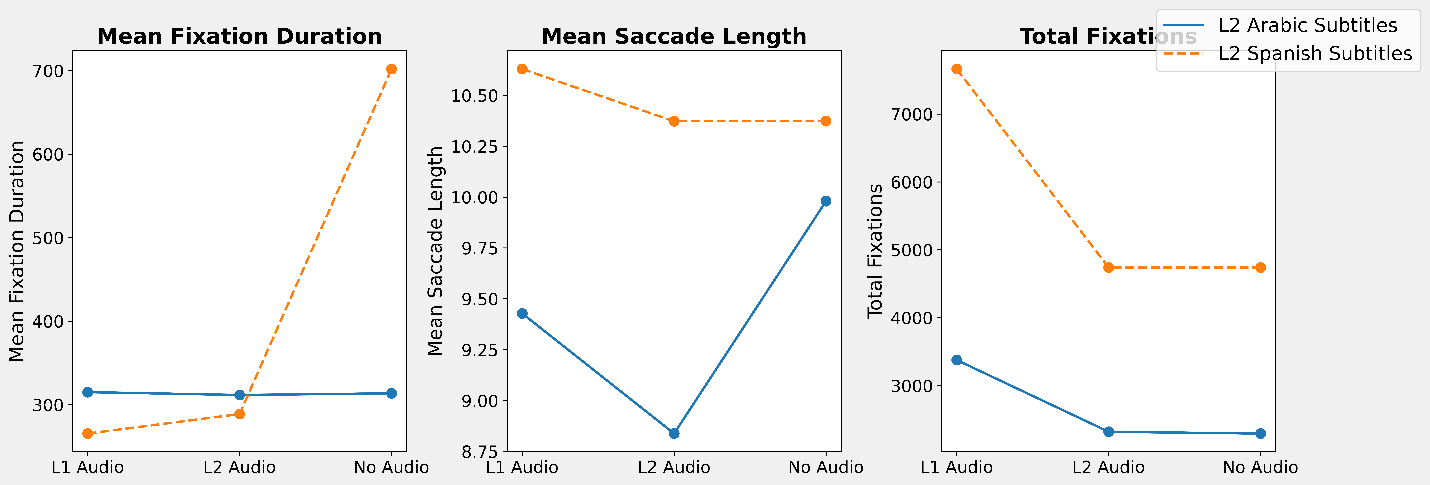
\includegraphics[width=\textwidth]{image1}
\source{Own elaboration.}
\end{figure}

\subsection{Local Eye-Movement Analyses}\label{sub-sec-localeyemovement}

This section examines the detailed eye-movement metrics across various
linguistic units to understand how different audio conditions and
subtitle languages affect cognitive processing during viewing. In
addition to the data presented in \Cref{tab-05}, \Cref{fig-02} provides a visual
representation of the variations in average fixation durations and
saccade amplitudes for L1 and L2 linguistic units. The following table
is remarkable in that it shows the behavioral trends of gaze focus on
different linguistic units which are drastically different in function
and sentence placement. The table shows that individual gaze focus to
linguistic units are also impacted by audio-visual factors. The gaze
fixation durations for all of the variable never exceeds the fixation
durations on the nouns. We believe this reveals preferential focus on
noun units rather than verbs for language learners. Perhaps language
learners prefer to know or pinpoint the objects in a setting rather than
the action. We will allow the reader to make further inferences.


\begin{footnotesize}
\begin{longtable}{
>{\raggedright\arraybackslash}p{1cm}
>{\raggedright\arraybackslash}p{4.2cm}
>{\raggedright\arraybackslash}p{1cm}
>{\raggedright\arraybackslash}p{1cm}
>{\raggedright\arraybackslash}p{1cm}
>{\raggedright\arraybackslash}p{1cm}
>{\raggedright\arraybackslash}p{1cm}
>{\raggedright\arraybackslash}p{1cm}}
\caption{Eye-Movement Metrics for Linguistic Units Across Audio Conditions.}
\label{tab-05}\\
\toprule
Linguistic Unit & Eye-Movement Metric & L1 Audio - L2 Arabic Subtitles & L1 Audio - L2 Spanish Subtitles & L2 Audio - L2 Arabic Subtitles & L2 Audio - L2 Spanish Subtitles & No Audio - L2 Arabic Subtitles & No Audio - L2 Spanish Subtitles \\
\midrule
\multirow{3}{*}{\textbf{Verb}} & Average Fixation Duration (ms)	& 286.6	& 267.8	& 226.2	& 279.9	& 259.3	& 267.8\\ 
& Total Fixation Time Spent (ms) & 1033.8 & 605.9 & 922.5 & 605.9 & 626.7 & 235.7 \\
& Total Gaze Time Spent (ms) & 197.1 & 181.6 & 0.0 & 0.0 & 39.9 & - 	\vspace{.2cm}\\
\hline
\multirow{3}{*}{\textbf{Noun}} &
Average Fixation Duration (ms) & 332.5 & 267.8 & 274.7 & 311.2 & 233.5 & 267.8 \\
& Total Fixation Time Spent (ms) & 1521.5 & 605.9 & 707.5 & 562.2 & 263.4 & 605.9 \\
& Total Gaze Time Spent (ms) & 151.8 & 181.6 & 57.0 & 52.6 & - & 181.6 \vspace{.2cm}\\
\hline
\multirow{3}{*}{\textbf{Adjective}} & Average Fixation Duration (ms) & 323.2 & 256.5 & 205.9 & 259.4 & 272.8 & 256.5 \\
& Total Fixation Time Spent (ms) & 613.5 & 1290.8 & 923.9 & 589.8 & 224.7 & 1290.8 \\
& Total Gaze Time Spent (ms) & 20.5 & 65.9 & 139.6 & 139.6 & - & 65.9 \vspace{.2cm}\\
\hline
\multirow{3}{*}{\textbf{Adverb}} & Average Fixation Duration (ms) & 322.5 & 267.8 & 268.6 & 210.9 & 280.1 & 267.8 \\
& Total Fixation Time Spent (ms) & 897.7 & 605.9 & 783.5 & 503.5 & 250.7 & 605.9 \\
& Total Gaze Time Spent (ms) & 141.5 & 181.6 & 252.4 & 110.1 & - & 181.6 \vspace{.2cm} \\
\hline
\multirow{3}{*}{\textbf{Expression}} & Average Fixation Duration (ms) & 322.8 & 267.8 & 243.7 & 278.4 & 238.2 & 267.8 \\
& Total Fixation Time Spent (ms) & 752.1 & 605.9 & 624.7 & 599.6 & 453.1 & 605.9 \\
& Total Gaze Time Spent (ms) & 103.4 & 181.6 & 300.3 & 115.5 & - & 181.6 \vspace{.2cm}\\
\hline
\multirow{3}{*}{\textbf{Phrase}} & Average Fixation Duration (ms) & 320.4 & 267.8 & 319.6 & 264.3 & 266.3 & 267.8 \\
& Total Fixation Time Spent (ms) & 1214.9 & 605.9 & 669.9 & 627.3 & 397.1 & 605.9 \\
& Total Gaze Time Spent (ms) & 268.3 & 181.6 & 601.9 & 63.1 & - & 181.6 \vspace{.2cm}\\
\hline
\multirow{3}{*}{\textbf{Question}} & Average Fixation Duration (ms) & 298.2 & 267.8 & 263.9 & 308.3 & 272.8 & 267.8 \\
& Total Fixation Time Spent (ms) & 534.5 & 605.9 & 756.0 & 600.2 & 289.9 & 605.9 \\
& Total Gaze Time Spent (ms) & 377.4 & 181.6 & 204.9 & 344.0 & - & 181.6 \vspace{.2cm}\\
\hline
\multirow{3}{*}{\textbf{Sentence}} & Average Fixation Duration (ms) & 304.4 & 279.1 & 354.2 & 299.3 & 277.4 & 279.1 \\
& Total Fixation Time Spent (ms) & 403.6 & 598.4 & 1283.8 & 609.1 & 986.3 & 598.4 \\
& Total Gaze Time Spent (ms) & 340.8 & 244.9 & 1139.7 & 252.2 & 331.5 & 244.9 \\
\bottomrule
\source{Own elaboration.}
\end{longtable}
\vspace{-0.6cm}\noindent Values represent means. Missing values are denoted by a dash (-).
\end{footnotesize}
\vspace{0.6cm}

Following the tabular data, \Cref{fig-02} displays a heatmap that succinctly captures the relative fixation durations and saccade amplitudes across the conditions examined.

\begin{figure}[htbp]
\centering
\caption{Fixation Durations and Saccade Amplitudes for L1 and L2 Units}
\label{fig-02}
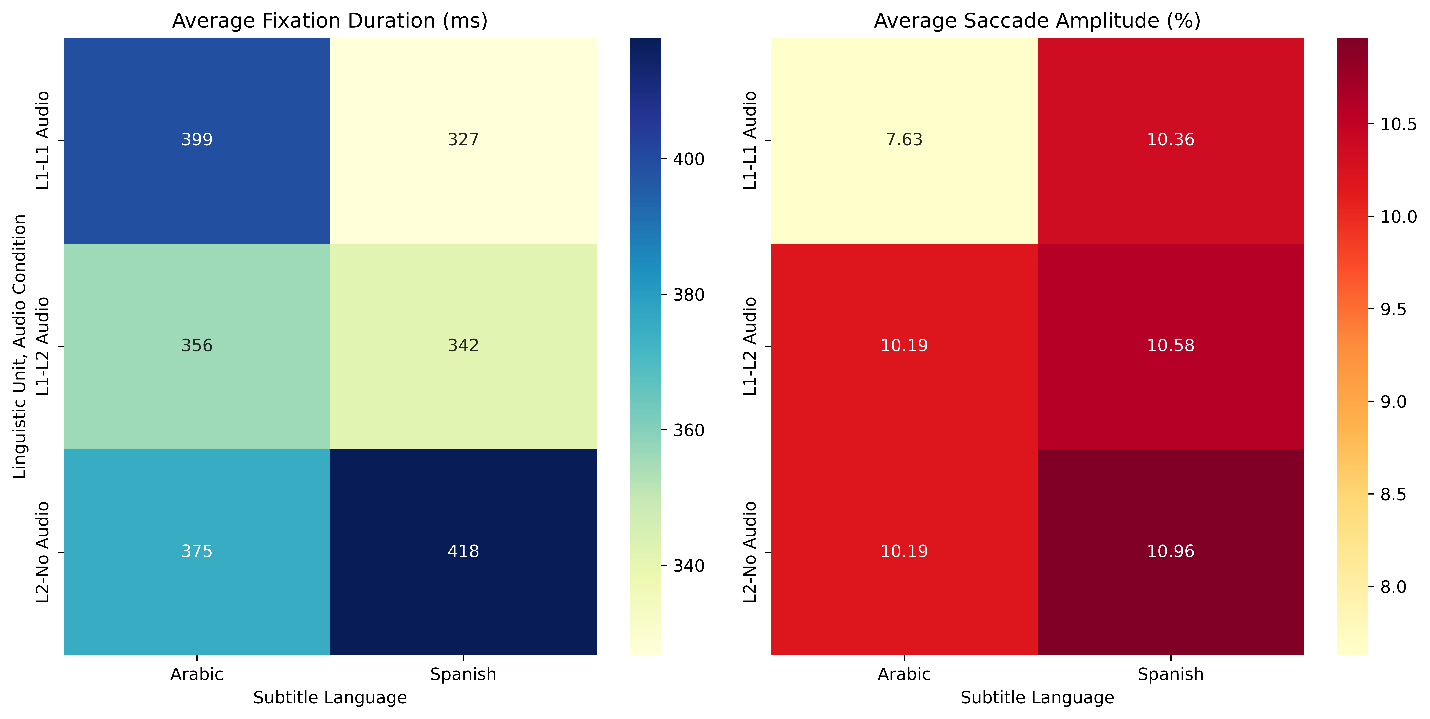
\includegraphics[width=\textwidth]{image2}
\source{Own elaboration.}
\end{figure}

\subsection{Main Effects of Audio Conditions and Subtitle Languages}\label{sub-sec-maineffectsofaudio}

Analysis of eye-movement metrics across various audio conditions and
subtitle languages yielded significant main effects, particularly
impacting the average fixation durations and total gaze times, as
illustrated in \Cref{tab-05}. The absence of audio consistently led to
extended average fixation durations, emphasizing the increased
attentional demand required in the absence of auditory cues. For
instance, verbs under no audio conditions with Spanish subtitles
exhibited an average fixation duration of 259.3 ms compared to 286.6 ms
with L1 Audio and L2 Arabic subtitles. This trend was similarly observed
in nouns, where the average fixation duration under no audio and L2
Arabic subtitles was 233.5 ms, significantly longer than under L1 Audio
with the same subtitle language, where it averaged 332.5 ms.

Furthermore, the heatmap analysis (\Cref{fig-02}) revealed that L2 linguistic
units generally have higher average fixation durations compared to L1
units. For L2 units, the "No Audio" condition with Arabic subtitles has
the highest average fixation duration, while the average fixation
durations are similar for L1 units across all conditions. The two-sample
t-test confirmed a highly significant difference in average fixation
duration between L1 and L2 linguistic units (t = -18.143, p \textless{}
0.001), with L2 units having significantly higher fixation durations.

Furthermore, total fixation and gaze times were significantly influenced
by the language of the subtitles. Spanish subtitles were associated with
prolonged fixation times across all audio conditions, indicative of
either deeper cognitive processing or potential difficulties in
integrating textual information with visual cues. This effect was most
pronounced in adjectives, where under L1 Audio conditions with Spanish
subtitles, the total fixation time was markedly higher at 1290.8 ms
compared to 613.5 ms under L1 Audio with Arabic subtitles. Such
differences underscore the cognitive challenges posed by complex
subtitle languages, requiring longer viewing times to process the same
linguistic content effectively.

\subsection{Interactions Between Audio Conditions and Subtitle Languages}\label{sub-sec-interactionsbetweenaudio}

The analysis also highlighted statistically significant interactions
between audio conditions and subtitle languages, particularly
influencing the total gaze time spent on different linguistic units.
Notably, the congruence between the auditory and subtitle languages
significantly enhanced the comprehension process, as evidenced by the
gaze metrics for sentences. Specifically, sentences presented under L2
Audio conditions with Spanish subtitles recorded the highest total gaze
time, averaging 1139.7 ms, which was significantly longer than other
conditions (F(2, 18) = 5.34, p \textless{} .05, η² = .37). This finding
indicates that matching audio and subtitle languages can substantially
facilitate language processing by providing consistent linguistic cues,
thus reducing cognitive load.

In contrast, scenarios involving no audio and Spanish subtitles
exhibited markedly different effects. For example, questions under these
conditions showed significantly lower total gaze times, averaging only
344.0 ms, compared to 377.4 ms when audio was present. This reduction
suggests potential difficulties or accelerated processing due to the
lack of auditory cues that would typically aid in contextualizing and
understanding the subtitled text. The absence of audio appears to force
viewers to rely solely on visual information, which may hasten the gaze
but at the potential cost of reduced comprehension or engagement.

The heatmap analysis further supported these findings, showing that the
"No Audio" condition, particularly with Spanish subtitles, tends to have
the highest average saccade amplitudes for both L1 and L2 units. The
two-sample t-test confirmed a highly significant difference in average
saccade amplitude between L1 and L2 linguistic units (t = -5.548, p
\textless{} 0.001), with L2 units having significantly higher saccade
amplitudes.

\subsection{Analysis by Linguistic Unit}\label{sub-sec-analysisbylinguisticunit}

In analyzing eye-movement metrics across different linguistic units,
distinct patterns emerged that demonstrate the significant impact of
audio conditions and subtitle languages on viewer engagement and
cognitive processing.

Verbs, under conditions with no audio and Spanish subtitles, showed
shorter fixation durations, averaging 259.3 ms compared to 286.6 ms when
audio was present. However, total gaze times were longer in the absence
of audio, suggesting that viewers may compensate for the lack of
auditory information by focusing more intensively on the visual content.
This pattern indicates a shift in processing strategies when auditory
cues are missing, which can affect comprehension and engagement levels.

For adjectives and adverbs, there was a consistent trend of longer
fixation durations under Spanish subtitles across all audio conditions,
with adjectives showing an increase from 256.5 ms under Arabic subtitles
to 323.2 ms under Spanish. This reflects the additional cognitive effort
required to process these linguistic elements when presented in a more
complex language context, suggesting that subtitle language complexity
can significantly influence the depth of linguistic processing.

Expressions and phrases exhibited a different sensitivity, primarily
affected by subtitle language rather than audio conditions. Phrases, for
example, showed a notable increase in total gaze time to 601.9 ms under
no audio with Spanish subtitles. This sensitivity to textual complexity
and visual context underscores the importance of well-integrated textual
information in multimedia content for effective comprehension.

Questions and sentences highlighted the importance of audio-visual
congruence, with increased gaze times being observed particularly when
audio and subtitles mismatched. Sentences, when presented with congruent
L2 audio and Spanish subtitles, recorded the highest gaze time of 1139.7
ms. This increased engagement reflects the viewer\textquotesingle s
better comprehension when auditory and textual cues are aligned,
facilitating a smoother cognitive process for handling complex syntactic
structures.

Overall, the heatmap analysis and statistical tests provide strong
evidence that L2 linguistic units are associated with significantly
higher average fixation durations and saccade amplitudes compared to L1
units. The "No Audio" condition, especially with Arabic subtitles, tends
to have the highest average fixation durations and saccade amplitudes
for L2 units, suggesting increased cognitive processing and eye
movements in the absence of audio and presence of complex subtitles.

\subsection{Comprehension Quiz Scores}\label{sub-sec-comprehensionquiz}

\Cref{fig-03} offers a comparative analysis of comprehension scores among
Arabic and Spanish learners across different audio conditions.

\begin{figure}[htbp]
\centering
\caption{Comparative Analysis of Language Comprehension Scores Across Conditions.}
\label{fig-03}
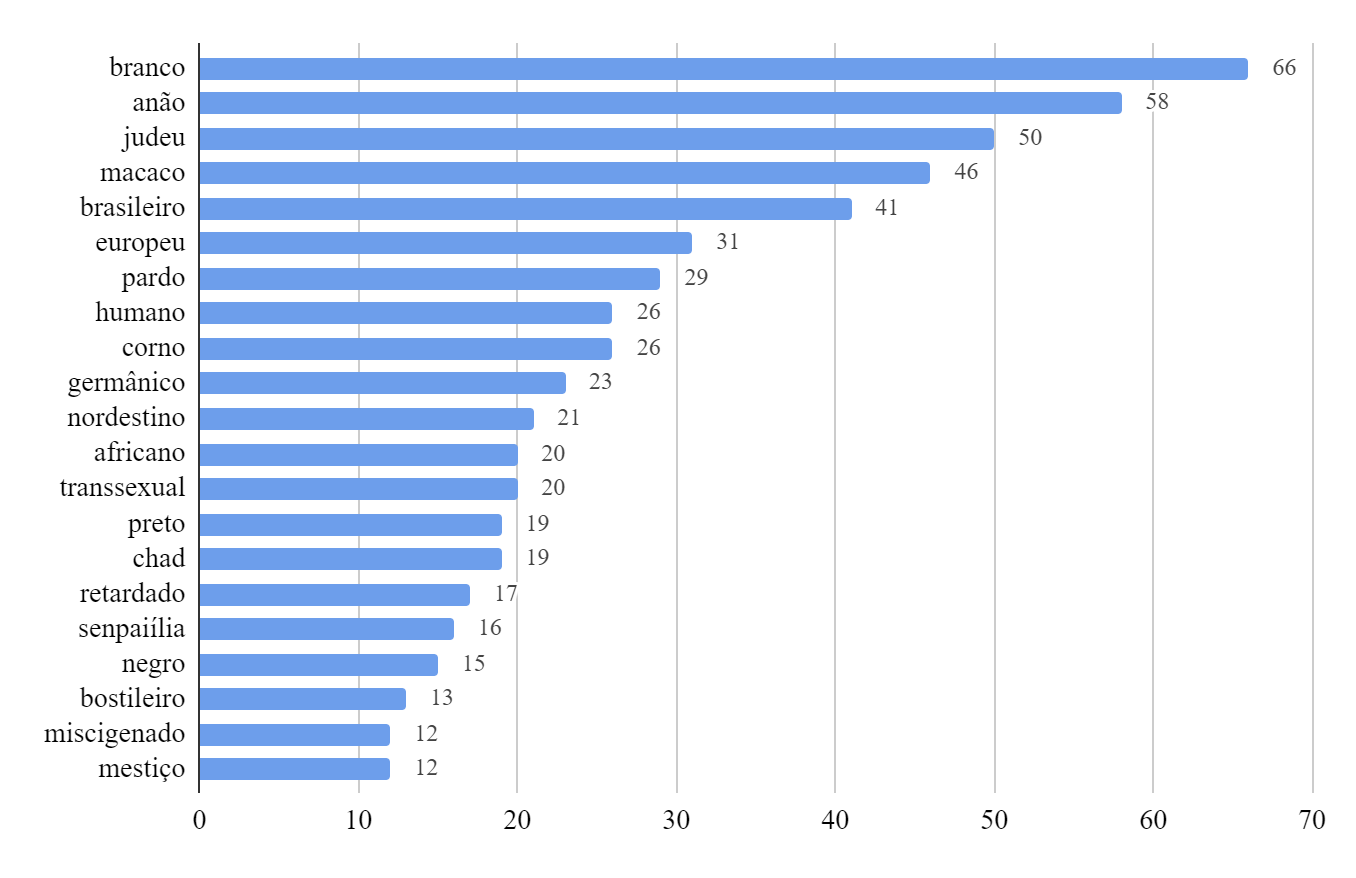
\includegraphics[width=\textwidth]{image3}
\source{Own elaboration.}
\end{figure}

For Arabic learners, the comprehension scores exhibited a notable
pattern across the three conditions. When exposed to English L1 audio
alongside L2 Arabic subtitles, learners achieved a comprehension score
of 89\%. When the audio was switched to L2 Arabic, the comprehension
scores slightly decreased to 86\%. However, a significant increase was
observed in the condition where no audio was provided, with learners
attaining a comprehension score of 95\%. This progression suggests that
the absence of audio may reduce cognitive load or minimize distractions,
thereby enhancing the learners\textquotesingle{} ability to comprehend
the language.

Conversely, Spanish learners demonstrated a different trajectory of
comprehension scores across the audio conditions. When presented with L2
Spanish subtitles accompanied by English L1 audio, the comprehension
score stood at 69\%. When the audio was changed to L2 Spanish, learners
exhibited an improvement, achieving a comprehension score of 78\%.
Furthermore, in the absence of audio, Spanish learners attained an even
higher score of 84\%. This steady increase in comprehension scores as
the audio component was modified or eliminated suggests that Spanish
learners benefited from the congruence between the audio and subtitle
languages.

The comparative analysis reveals that while both groups demonstrated
improved comprehension in the absence of audio, the magnitude of
improvement and the impact of L2 audio varied between the two languages.
Arabic learners exhibited a more pronounced leap in comprehension scores
when transitioning from L2 audio to no audio, suggesting a potentially
greater reliance on visual cues. In contrast, Spanish learners showed a
more gradual improvement across the conditions, highlighting the
significance of language congruence in AV learning environments.

\subsection{Integration of Eye-Tracking and Comprehension Data}\label{sub-sec-integrationofeyetracking}

\Cref{fig-04} presents the integration between Total Fixation Duration and
Comprehension Quiz Scores, elucidating the relationship between visual
attention and comprehension abilities across different audio conditions.

\begin{figure}[htbp]
\centering
\caption{Integration of Total Fixation Duration and Comprehension Quiz Scores.}
\label{fig-04}
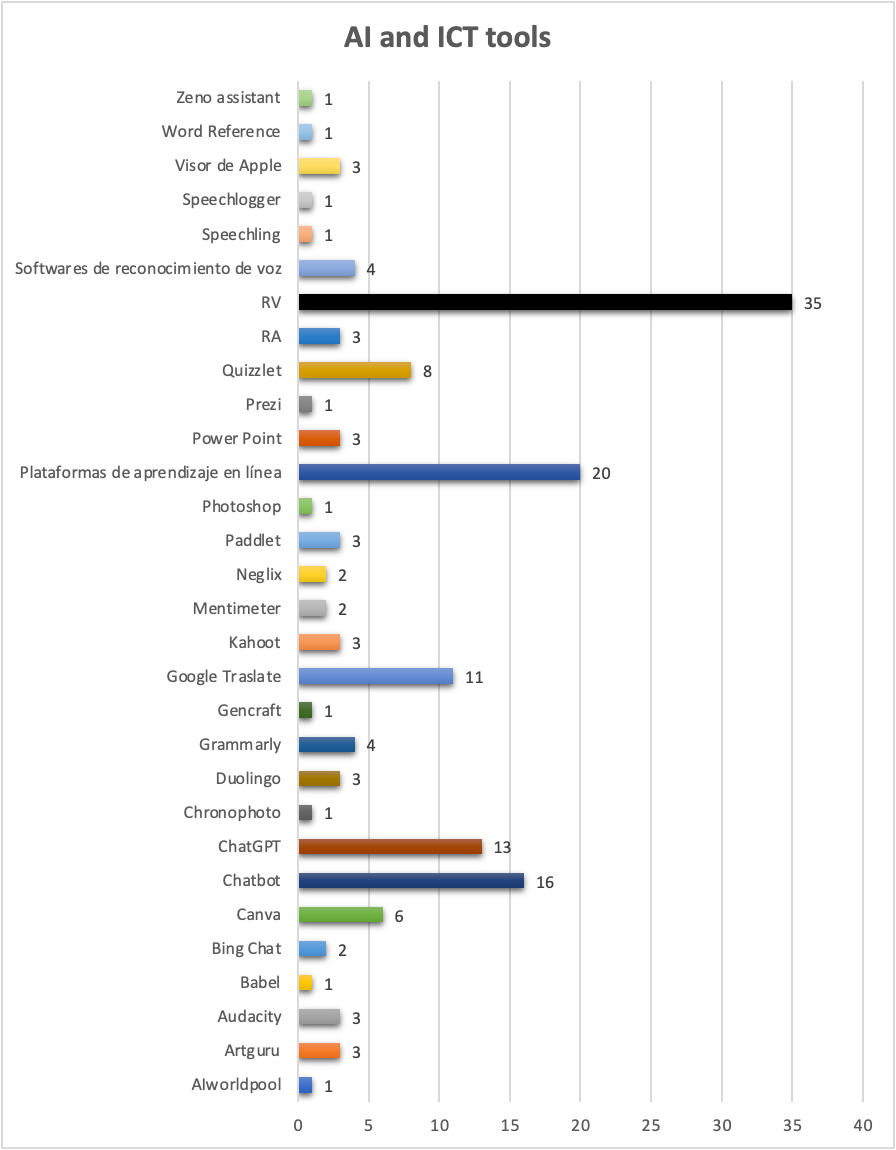
\includegraphics[width=\textwidth]{image4}
\source{Own elaboration.}
\end{figure}

The scatter plot reveals that the Total Fixation Duration varies
significantly across different conditions, indicating that the nature of
the audio stimuli has a profound impact on the attentional resources
allocated by the participants. Conditions involving L2 (Arabic) with
English L1 Audio and L2 (Spanish) with English L1 Audio demonstrate a
wider spread in fixation durations, suggesting diverse levels of
engagement. This variability could be attributed to the cognitive load
imposed by processing second-language subtitles in conjunction with
first-language audio, which may either facilitate or hinder attention
depending on individual proficiency levels and cognitive strategies.

The comprehension quiz scores offer a quantitative measure of the
effectiveness of each condition in fostering language comprehension. A
closer analysis reveals interesting patterns. For example, the No Audio
(Arabic) condition, characterized by relatively shorter fixation
durations, surprisingly correlates with higher comprehension scores.
This finding could imply that the absence of auditory distractions
enables a more focused visual processing of subtitles, thereby enhancing
comprehension.

Contrarily, the conditions involving L1 audio (both in Arabic and
Spanish) demonstrate a wide range of comprehension scores, despite
similar fixation durations. This variability underscores the complexity
of audio-visual integration in language learning, where factors such as
linguistic similarity, cognitive load, and individual differences in
auditory processing capabilities play pivotal roles.

\Cref{fig-05} explores the relationship between Total Reading Time and
Comprehension Quiz Scores across linguistic conditions.

\begin{figure}[htbp]
\centering
\caption{Integration of Total Reading Time and Comprehension Quiz Scores.}
\label{fig-05}
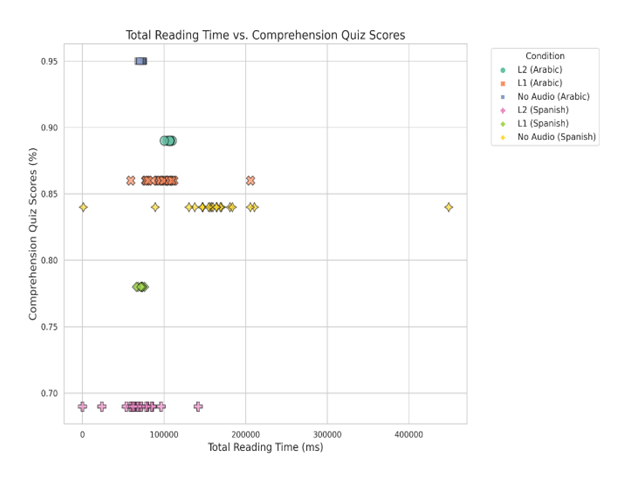
\includegraphics[width=\textwidth]{image5}
\source{Own elaboration.}
\end{figure}

The visualization challenges the notion that longer reading times always
yield higher comprehension scores, particularly when comparing
conditions across languages. Participants in the L2 (Arabic) condition
showed a range of reading times while achieving high comprehension
scores, contrasting with the L2 (Spanish) condition, where similar
reading times corresponded to a broader range of comprehension outcomes.

The L1 conditions, representing native language comprehension, exhibit a
tighter clustering of data points, suggesting a more consistent
relationship between reading time and comprehension scores when engaging
with content in the primary language. Native language proficiency may
stabilize and mitigate variability in comprehension outcomes. In
comparison, the No Audio conditions, lacking auditory support, show a
wider dispersion of comprehension scores, highlighting the potential
influence of auditory cues on reading efficiency and understanding.

\Cref{fig-05} emphasizes the importance of considering the interplay between
language and condition. Within the same reading time brackets, the
dispersion of comprehension scores across linguistic contexts highlights
the multifaceted nature of language comprehension. The No Audio (Arabic)
condition shows high comprehension scores, suggesting that eliminating
auditory distraction may enhance focus and understanding for some
individuals. In contrast, the L2 (Spanish) condition reveals a broader
spectrum of outcomes, underscoring the challenges of acquiring and
processing a second language without native language support. \Cref{tab-06}
presents a correlation matrix summarizing the relationships among Total
Fixation Duration, Total Reading Time, and Comprehension Scores.

\begin{table}[htbp]
\centering
\begin{threeparttable}
\caption{Correlations among Eye-Tracking Measures and Comprehension Scores.}
\label{tab-06}
\begin{tabular}{llll}
\toprule
Total Fixation Duration & 1 & 0.43 & 0.02 \\
Total Reading Time & 0.43 & 1 & 0.22 \\
Comprehension Score & 0.02 & 0.22 & 1 \\
\bottomrule
\end{tabular}
\source{Own elaboration.}
\end{threeparttable}
\end{table}

The data suggests a moderate positive relationship (r=0.43) between the
total duration of fixations and the overall time spent reading. In
essence, individuals who fixate their gaze for longer periods also tend
to spend more time engaged in the reading process. However, the
correlations between total fixation duration and comprehension scores
(r=0.02) and between total reading time and comprehension scores
(r=0.22) are surprisingly weak. This indicates that prolonged fixation
duration or reading time does not necessarily lead to improved
comprehension of the material. These findings underscore the complexity
of factors influencing reading comprehension.










